\documentclass[twocolumn,amsmath,amssymb,floatfix]{revtex4}

\usepackage{graphicx}% Include figure files
\usepackage{dcolumn}% Align table columns on decimal point
\usepackage{bm}% bold math
\usepackage{amssymb}
\usepackage{amsmath}
\usepackage{amsfonts}
\usepackage{epsf}
\usepackage{color} % allows color in fonts
\usepackage{verbatim}
\usepackage{listings}
\usepackage{xcolor}
\usepackage{titlesec}
\usepackage{float}

\usepackage[brazilian]{babel}
\usepackage[utf8]{inputenc}
\usepackage[T1]{fontenc}

\newcommand{\PAR}[1]{\left({[#1]}\right)}


\lstdefinestyle{customc}{
  belowcaptionskip=1\baselineskip,
  breaklines=true,
  frame=none,
  xleftmargin=\parindent,
  language=C,
  showstringspaces=false,
  basicstyle=\footnotesize\ttfamily,
  keywordstyle=\bfseries\color{green!40!black},
  commentstyle=\itshape\color{purple!40!black},
  identifierstyle=\color{blue},
  stringstyle=\color{orange},
}

\lstdefinestyle{customasm}{
  belowcaptionskip=1\baselineskip,
  frame=trBL,
  xleftmargin=\parindent,
  language=[x86masm]Assembler,
  basicstyle=\footnotesize\ttfamily,
  commentstyle=\itshape\color{purple!40!black},
}

\lstset{escapechar=@,style=customc}

\titlespacing\section{0pt}{12pt plus 4pt minus 2pt}{8pt plus 2pt minus 2pt}
\titlespacing\subsection{0pt}{12pt plus 4pt minus 2pt}{8pt plus 2pt minus 2pt}
\titlespacing\subsubsection{0pt}{12pt plus 4pt minus 2pt}{0pt plus 2pt minus 2pt}

\begin{document}

%%%%%%%%%%%%%%%%%%%%%%
%%%%%%%%%%%%%%%%%%%%%%
% T I T U L O
%%%%%%%%%%%%%%%%%%%%%%
%%%%%%%%%%%%%%%%%%%%%%

\title{Relatorio Exercicio Computacional 1}

\author{Leonardo Heidi Almeida Murakami - NUSP: 11260186 \\\small leonardo.murakami@usp.br} 
\affiliation{
Instituto de Matemática e Estatística - Universidade de São Paulo\\
}

\begin{abstract}
\baselineskip 11pt
Neste trabalho utilizaremos o método de Monte Carlo, que consiste em amostragens aleatórias massivas para obter resultados numéricos, para estimarmos o valor de $\pi$ (Pi), foi estudado nesse trabalho o erro variando-se o valor de $n$.
\end{abstract}

\maketitle
%%%%%%%%%%%%%%%%%%%%%%
%%%%%%%%%%%%%%%%%%%%%%
\section{Introdução e Conceitos}
%%%%%%%%%%%%%%%%%%%%%%
%%%%%%%%%%%%%%%%%%%%%%

\indent Os métodos de Monte Carlo são uma classe ampla de algoritmos computacionais que dependem de uma amostragem aleatória para obter resultados numéricos. 
\\\indent A ideia para obtermos o valor de $\pi$ será gerarmos pontos aleatórios (x, y) num plano 2-D com domínio pertencente a um quadrado de 1 unidade de lado.
\\\indent Após gerarmos os $n$ pontos aleatórios, calculamos a área do circulo como a proporção
\begin{eqnarray}
  p = \frac{1}{n}\sum_{i=1}^{n}T(x_i)
  \\
  T(x) = Ind(||x||_2 \leq 1) 
\end{eqnarray}
ou seja, a proporção de pontos que caíram dentro do círculo, sobre a quantidade de pontos totais, conseguimos então uma estimativa da areá do circulo.
\\\indent Como sabemos que o raio do círculo será de meia unidade, teremos que
\begin{eqnarray}
  p \approx \frac{area \ do \ circulo}{area \ do \ quadrado} = \frac{\pi * (\frac{1}{2})^2}{1}
  \\
  \pi \approx 4p
\end{eqnarray}
\\\indent Para calcularmos um erro que não dependesse do próprio $\pi$ utilizei o desvio padrão calculado após $m$ simulações sob o mesmo $n$. O Pi retornado será a média de $m$ simulações (logo, o número real de números aleatórios gerados será de $n*m$)
%%%%%%%%%%%%%%%%%%%%%%
%%%%%%%%%%%%%%%%%%%%%%
\section{Implementação e testes}
%%%%%%%%%%%%%%%%%%%%%%
%%%%%%%%%%%%%%%%%%%%%%

O algoritmo foi implementado na linguagem Python, organizado em 1 arquivo: monte-carlo-pi.py. Os gráficos foram
gerados usando a biblioteca \textit{matplotlib} do Python. As partes relevantes dos códigos podem ser
conferidos no próprio arquivo enviado junto com este PDF/Tex.

%%%%%%%%%%%%%%%%%%%%%%
\subsection{Arquivos do projeto}
%%%%%%%%%%%%%%%%%%%%%%
Abaixo segue um breve resumo do conteúdo dos códigos fonte e interfaces.
\\\indent \textbf{monte-carlo-pi.py:} Implementa todo o algoritmo. Um pedaço de sua interface é apresentado a seguir:
\begin{lstlisting}
def get_point() -> Tuple(float, float):

def vector_module(vector_components: Tuple(float, float) -> float:

def calculate_pi(n_samples: int) -> float:

def early_stopping(target_error: float, iteration_m: int = 300) -> float:

def main() -> float
\end{lstlisting}
A função early stopping, que possui o nome menos direto, aumenta o numero de $n$ até que o desvio padrão percentual calculado seja menor que o erro passado como parâmetro, para cada tentativa esta função aumentará em 10 vezes o valor anterior de $n$. Como indicado na enunciação do problema, utilizaremos na \textbf{main()} um valor de $0.05\%$ de erro para calcularmos pi. 
%%%%%%%%%%%%%%%%%%%%%%
\subsection{Algoritmo}
%%%%%%%%%%%%%%%%%%%%%%
A implementação do algoritmo em questão é apresentado abaixo. A função calculate\_pi recebe como argumento n\_samples, que condiz com o $n$ anteriormente citado. A função early\_stopping utiliza-se desta função e recebe o valor de erro que deseja-se atingir, assim como recebe $m$, a quantidade de valores estimados de pi que devem ser calculados com aquele valor de $n$.
\\\indent Afim de evitar um consumo muito grande de memória (que possibilitaria testes com valores muito grandes de $n$) atualizamos o valor de T conforme geramos os pontos, dessa maneira, evitamos guardar os pontos numa lista.
\begin{lstlisting}
def calculate_pi(n_samples):
  sum_T = 0
  for i in range(n_samples):
      if vector_module(get_point()) <= CIRCLE_RADIUS:
          sum_T+=1
  #calculate proportion given in the exercise
  proportion = (1/n_samples)*sum_T
  #return 
  return proportion*4

def early_stopping(target_error, iteration_m=300):
    n_samples = 1
    percentage_error = 1
    while percentage_error > target_error:
      calculated_pis = [calculate_pi(n_samples) for i in range(iteration_m)]
      std_error = pstdev(calculated_pis)/sqrt(iteration_m)
      percentage_error = (std_error/mean(calculated_pis))*100
      n_samples*=10

      print("---------------------------")
      print(f"NUM SAMPLES:\t{n_samples}")
      print(f"STD ERROR:\t{std_error}")
      print(f"PERCENTAGE ERROR:\t{percentage_error}")
      print(f"ESTIMATED AVERAGE PI:\t{mean(calculated_pis)}")
      print("---------------------------")

    return mean(calculated_pis)
\end{lstlisting}
A função early\_stopping possui diversos comandos de \textit{print} afim de possibilitar ver o progresso de cada \textit{batch} de proporções calculadas, rodamos este algoritmo até atingir um valor de percentage\_error menor que o erro alvo, podemos então retornar a média dos $m$ $\pi$s calculados

%%%%%%%%%%%%%%%%%%%%%%
\subsection{Testes}
%%%%%%%%%%%%%%%%%%%%%%
Para validar o código numericamente, fiz alguns testes manuais que mostravam valores muito próximos do valor real de $\pi$.

%%%%%%%%%%%%%%%%%%%%%%
\subsection{Valor ideal de N}
%%%%%%%%%%%%%%%%%%%%%%
Existe uma relação inversa entre o peso computacional e a precisão de $\pi$ calculada por este algoritmo. Embora para valores muito grandes de $n$ possuamos uma precisão maior, estes podem demorar muito tempo para serem executados, de tal modo que possa ser mais vantajoso utilizar um $n$ menor.
\\\indent Embora a função early\_stopping calcule esse $n$ ideal dado a precisão necessária, é possível visualizar a diminuição do erro saturar ao aumentar de números aleatórios gerados
\\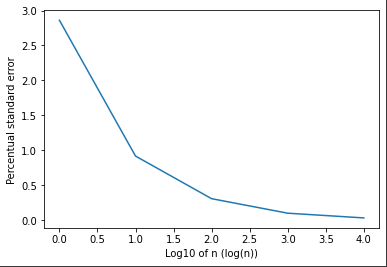
\includegraphics[scale=0.85]{prct_std_error.png}
\\\indent Para fins de melhor entendimento, considere $N = m*n$, para a faixa de precisão dada pelo enunciado do problema, podemos utilizar $N = 3000000$
\end{document}